% \section{Architettura del sistema}
% \subsection{Componenti}
% \begin{frame}
%   \frametitle{Componenti di un software di riconoscimento della respirazione}
%   
% % In generale un sistema che riconosce la respirazione a partire da alcuni segnali fisiologici continui, deve essere sensibile al cambiamento di alcune caratteristiche del segnale che sono omomorfe alla presenza, al volume, al flusso o alla frequenza della respirazione. 
% % Queste caratteristiche sono in generale dipendenti dal contesto quindi ci aspettiamo che un buon algoritmo faccia leva su delle quantit\`a statistiche del segnale o su una qualche forma di apprendimento automatico. 
% % Ci aspettiamo anche che tali caratteristiche rispettino un qualche principio di localit\`a questo perch\'e le propriet\`a della respirazione cambiano molto nel lungo termine.
% 
% % La figura \ref{schemaGeneraleAlg} mostra uno schema generale nel quale rientrano tutti i possibili sistemi software di riconoscimento della respirazione attraverso dei sensori.
% \begin{figure}
%  \centering
%  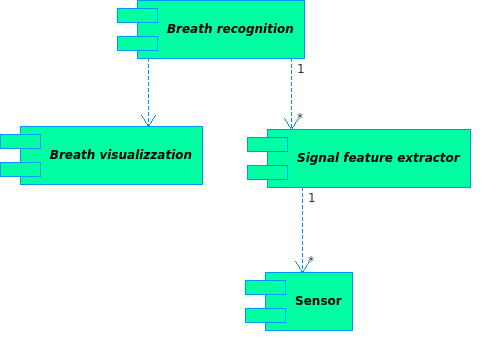
\includegraphics[width=0.9\textwidth]{./metodologiaDiagramma.png}
% \end{figure}
% \end{frame}


\section{Architettura del sistema}
\subsection{Schema di funzionamento}
\begin{frame}
  \frametitle{Schema di funzionamento}
\begin{center}
\begin{tikzpicture}
%   [scale=.8,auto=left,every node/.style={fill=blue!20}]
[->,>=stealth',shorten >=1pt,auto,node distance=3cm,
  thick,main node/.style={circle,fill=blue!20,draw,font=\sffamily\LARGE\bfseries},
  decision node/.style={draw,font=\sffamily}]

  \node [main node] (start) at 			(2,5.5) 	{};
  \node  (Acquisizione) at 			(2,4.5) 	{Acquisizione dati dallo stetoscopio elettronico};
  \node (Estrazione) at 			(2,3.5)	{Estrazione dei suoni respiratori};
  \node (Riconoscimento) at 			(2,2.5) 	{Riconoscimento delle apnee};
  \node [decision node] (Apnea) at 		(2,1.5) 	{Durata totale delle ultime apnee consecutive $>$ soglia di rischio?};
  \node  (Allarme) at				(4,0) 	{Allarme};
  \node [main node] (end) at 			(0,0) 	{};	

   \foreach \from/\to in {start/Acquisizione,Acquisizione/Estrazione,Estrazione/Riconoscimento,Riconoscimento/Apnea}
     \draw (\from) -- (\to);

 \draw[every node/.style={font=\sffamily\small}]
     (Apnea) edge node [left] {si} (Allarme)
     (Apnea) edge node [right] {no} (end);

\end{tikzpicture}
\end{center}
\end{frame}
